\documentclass[]{article}

\usepackage{setspace}
\usepackage{amsmath}
\usepackage{amssymb}
\usepackage{graphicx}
\usepackage[a4paper,top=2cm,bottom=3cm,left=4cm,right=4cm]{geometry}
\usepackage{caption}
\usepackage[svgnames]{xcolor}
\usepackage{listings}

\lstset{language=R,
	basicstyle=\small\ttfamily,
	stringstyle=\color{DarkGreen},
	otherkeywords={0,1,2,3,4,5,6,7,8,9},
	morekeywords={TRUE,FALSE},
	deletekeywords={data,frame,length,as,character},
	keywordstyle=\color{blue},
	commentstyle=\color{DarkGreen},
}


\renewcommand{\baselinestretch}{1.5} 

%opening
\title{Statistical arbitrage strategies : from static to time-varying approaches }
\author{Minichini Carmine}
\date{}

\begin{document}
\maketitle


\begin{abstract}

\end{abstract}

%%%%%%%%%%%%%%%
% TEORIA
%%%%%%%%%%%%%%%
\section{Teoria}

\subsection{Co-integration}
Per introdurre il concetto di co-integrazione tra due serie temporali è utile definire il concetto di integrazione.
\\
Una serie temporale $X_t$ è definita integrata di ordine 1, $I(1)$, se non è stazionaria, ma è stazionaria nelle prime differenze $X_t - X_{t-1}$.
\\
Il concetto di co-integrazione prende invece in esame due serie temporali: \\ due serie temporali $X_t$ e $Y_t$ integrate di ordine $I(1)$, sono co-integrate se la loro combinazione lineare è un processo debolmente stazionario.

\begin{equation} 
	\hat{\epsilon} = Y_t - \hat{\beta}X_t - \hat{\alpha}
\end{equation}
\\
Seguendo l'approccio two-step Engle-Granger(1987), per verificare la stazionarietà del processo $\hat{\epsilon_t}$, dopo aver stimato $\alpha$ e $\beta$ con una regressione lineare , si testa la presenza di una radice unitaria tramite il test aumentato di Dickey-Fuller (ADF).

\subsection{Linear State Space Models}

Gli State Space Models (Modelli nello Spazio degli Stati) forniscono una metodologia generale di riferimento, molto flessibile, per affrontare una vasta gamma di problemi nell’analisi delle serie storiche.
L’idea metodologica alla base degli State Space Models è che lo
sviluppo nel tempo del fenomeno in analisi, $y_1....y_n$ , sia determinato da una serie di vettori non osservabili $\theta_1....\theta_n$.
La relazione tra $y_t$ e $\theta_t$ specifica il modello nella forma state space.

\subsubsection{Time-varying coefficients}
La relazione lineare tra due variabili co-integrate è descritta da:
\begin{equation}\label{classic_cointegration}
	y_t = \alpha + \beta x_t + \epsilon_t
\end{equation}
\\
In cui $\alpha$ e $\beta$ sono invarianti nel tempo.
La formulazione dell'equazione \ref{classic_cointegration} come un modello state space Gaussiano ci permette di considerare invece l'evoluzione degli stati $\alpha$ e $\beta$ nel tempo. Assumendo che questi si evolvano secondo un processo random walk avremo che \footnote{J. Durbin and S. J. Koopman, Time Series Analysis by State Space Methods, 2nd Ed. Oxford University Press, 2012}:
\begin{align}
	y_t = \alpha_t + \beta_t x_t + \epsilon_t\\
	\alpha_t = \alpha_{t-1} + \eta_{1,t}\\        
	\beta_t = \beta_{t-1} + \eta_{2,t}
\end{align}
\\
Il modello state space gaussiano è quindi definito da due equazioni\footnote{Daniel P. Palomar- Portfolio Optimization with R - The Hong Kong University of Science and Technology (HKUST)}:
\begin{align}
		\theta_{t+1}=T_t\theta_t + \eta_t\\   
		y_t = Z_t\theta_t + \epsilon_t 
\end{align}

\begin{itemize}
	\item $\theta_t \triangleq \begin{bmatrix}
		\alpha\\
		\beta
	\end{bmatrix}$ è lo stato inosservato
	
	\item $T_t \triangleq \begin{bmatrix}
		1 & 0 \\
		0 & 1
	\end{bmatrix}$ è la matrice di transizione degli stati
	
	\item $\eta_t \sim \mathcal{N}(0,Q)$ è detto \textbf{state transition noise} ed è un errore gaussiano a media 0 e con matrice di covarianza $Q \triangleq \begin{bmatrix}
		\sigma^2_1 & 0 \\
		0 & 	\sigma^2_2
	\end{bmatrix}$
	
	\item $Z_t \triangleq  \begin{bmatrix}
		1 & x_t
	\end{bmatrix}$ è la matrice di osservazione, dove $x_t$ rappresenta,nel nostro caso,un vettore di prezzi.
	
	\item $\epsilon_t \sim \mathcal{N}(0,\sigma^2_e)$ è detto \textbf{observation noise} 
\end{itemize}
\
\\
L'equazione (6) è definita \textbf{equazione di transizione} ed esprime la transizione dello stato $\theta_t$ attraverso una relazione lineare.
\\
L'equazione (7) è invece definita \textbf{equazione di misurazione} ed esprime la relazione lineare tra lo stato di osservazioni $y_t$ e lo stato latente $\theta_t$.
\\
Una volta specificato il modello in forma state space, la stima degli stati inosservati $\theta$ può essere ottenuta in maniera ricorsiva attraverso l'utilizzo di un Kalman Filter.
\\
\subsubsection{Inizializzazione del Kalman Filter}
Il modello definito dalle equazioni (6) e (7) viene inizializzato con l'ipotesi base che i  parametri $\sigma^2_1,\sigma^2_2$ ,responsabili dell'incertezza attorno all'evoluzione stocastica dello stato $\theta$, siano di ordine molto piccolo, prossimo allo zero.
L'ipotesi base con cui viene inizializzato il modello è quindi di assumere $\sigma^2_1=0.0001, \sigma^2_2=\sigma^2_1,  \sigma^2_e=0.001$.

%%%%%%%%%%%
% ANALISI SPERIMENTALE
%%%%%%%%%%%

\section{Dati e metodologie}
L'analisi empirica è stata svolta considerando i prezzi di chiusura giornalieri, aggiustati per i dividendi, dei costituenti dell'indice FTSE MiB nel periodo dal 1° gennaio 2015 al 31 dicembre 2019.\footnote{I prezzi di chiusura giornalieri, aggiustati per i dividendi, sono stati ottenuti tramite Yahoo Finance}
Il campione ottenuto è stato poi diviso in:
\begin{itemize}
	\item \textbf{Periodo di Training}: Dal 1° gennaio 2015 al 31 dicembre 2018 (4 anni)
	\item \textbf{Periodo di Testing}:  Dal 1° gennaio 2019 al 31 dicembre 2019 (1 anno)
\end{itemize}
\
L'analisi procede come segue:

\begin{enumerate}
	
	\item \textbf{Cointegration Test:} Nel periodo di training, per i 40 titoli dell'indice è stata testata la relazione di co-integrazione tramite il metodo two-step Engle-Granger.
	
	\item \textbf{Pairs Selection:} Stimata la relazione di co-integrazione, escluse le coppie non co-integrate,sono state selezionate le coppie dello stesso settore di appartenenza e ordinate per l'indice di correlazione di Pearson.
	
	\item \textbf{Statistical Arbitrage}: Nel periodo di testing, sono state implementate le 3 diverse strategie di trading.
	
	\item \textbf{Performance}: Valutazione della performance
\end{enumerate}

\subsection{Risultati della selezione}


\begin{center}
\captionof{table}{Risultati}\label{sophisticatedtable}
\begin{tabular}{ p{4cm}p{1cm}p{2cm}p{1cm}p{3cm} }
	\hline
	Pair & $\rho$ & ADF Statistic & p-value & Settore\\
	\hline
	DIA.MI - AMP.MI  & 0.97  & -3.66 &  0.026 & Sanitario\\
	UCG.MI - BPE.MI & 0.94 & -3.73 & 0.022 & Bancario\\
	BMED.MI - BGN.MI & 0.80 & -4.43 & 0.01 & Servizi Finanziari \\
	BMED.MI - AZM.MI  & 0.61 & -3.98 & 0.01 & Servizi Finanziari\\
	\hline
\end{tabular}
\end{center}

\section{Statistical Arbitrage}
Per il periodo di testing sono state considerate 3 strategie di trading, la prima basata sull'approccio classico di co-integrazione, in cui è stato calcolato lo spread con le stime dei parametri ottenuti tramite la regressione lineare nel periodo di training.
La seconda metodologia utilizzata prevede la stima, a intervalli regolari di 2 mesi, dei coefficienti $\hat{\alpha}$ e $\hat{\beta}$ nel periodo di testing, i parametri stimati nella finestra precedente sono stati poi utilizzati per calcolare lo spread nella finestra successiva. 
Il terzo approccio prevede una stima dinamica dei parametri $\alpha$ e $\beta $ attraverso l'utilizzo di un Kalman Filter.
Calcoliamo lo spread tra le due serie considerate nel periodo di testing come:
\begin{equation} 
	z_t= log(stock_{1,t}) - \hat{\beta}log(stock_{2,t}) - \hat{\alpha} \label{spread}
\end{equation}
\\
Gatev et al.(2006)\footnote{Gatev, E., Goetzmann,W. and Rouwenhorst, K. Pairs Trading: Performance of a Relative-Value Arbitrage Rule, Review of Financial Studies 19(3), 797–827. 2006} nel loro lavoro, adottano come threshold per una strategia di Pairs Trading un valore pari a 2 volte la deviazione standard dello spread calcolato nel periodo di training. 
Tuttavia un problema dell'adottare una threshold con l'approccio di Gatev et al. risiede nel considerare una soglia eccessivamente alta per le oscillazioni nel periodo di testing, portandoci nella maggior parte dei casi a non avere segnali di entrata o uscita.
Nella nostra casistica è stato scelto quindi di adottare una valore soglia costante per tutte le metodologie sviluppate, con due scopi: generare segnali molto aggressivi e riuscire ad equiparare le performance per tutti i modelli.
\\
I segnali per la strategia ($\pm 1$) sono così generati:
\begin{itemize}
	\item Se : $z_t > threshold$ . significa che $stock_{1,t}$ è sopravvalutato rispetto a $stock_{2,t}$, per cui vendiamo 1 unità di $stock_{1,t}$ e compriamo $\hat{\beta}$ unità di $stock_{2,t}$
	Chiudiamo la posizione quando $z_t\leq 0$
	\item Se: $z_t < - threshold$ . significa che $stock_{1,t}$ è sottovalutato rispetto a $stock_{2,t}$, per cui compriamo 1 unità di $stock_{2,t}$ e vendiamo $\hat{\beta}$ unità di $stock_{1,t}$
	Chiudiamo la posizione quando $z_t\geq 0$
\end{itemize}
\
L'intera strategia di trading è equivalente ad avere un portafoglio con pesi\footnote{Yiyong Feng and Daniel P. Palomar (2016), "A Signal Processing Perspective on Financial Engineering"}
\begin{equation} 
w\triangleq 
\begin{bmatrix}
	1 \\
	-\hat{\beta}
\end{bmatrix}
\end{equation}
\
sotto il vincolo che $w=1$ il portafoglio costruito per la strategia è :

\begin{equation} 
w\triangleq \begin{bmatrix}
	1/(1 + \hat{\beta}) \\
	-\hat{\beta}/(1 + \hat{\beta})
\end{bmatrix}
\end{equation}
\
mentre i ritorni del portafoglio considerato sono stati poi calcolati come:
\begin{equation}
	w^T\Delta log(stocks)
\end{equation}

\section{Performance}
La prima coppia considerata è formata dalle multinazionali \textbf{DiaSorin S.p.A.} e  \textbf{Amplifon S.p.A.}, entrambe operanti nel settore medico-sanitario.
\\
La figure 1 e 2 mostrano i parametri $\hat{\alpha}$ e $\hat{\beta}$ stimati con le tre metodologie:
\begin{figure}[h]
	\caption{$\hat{\alpha}$}
	\centering
	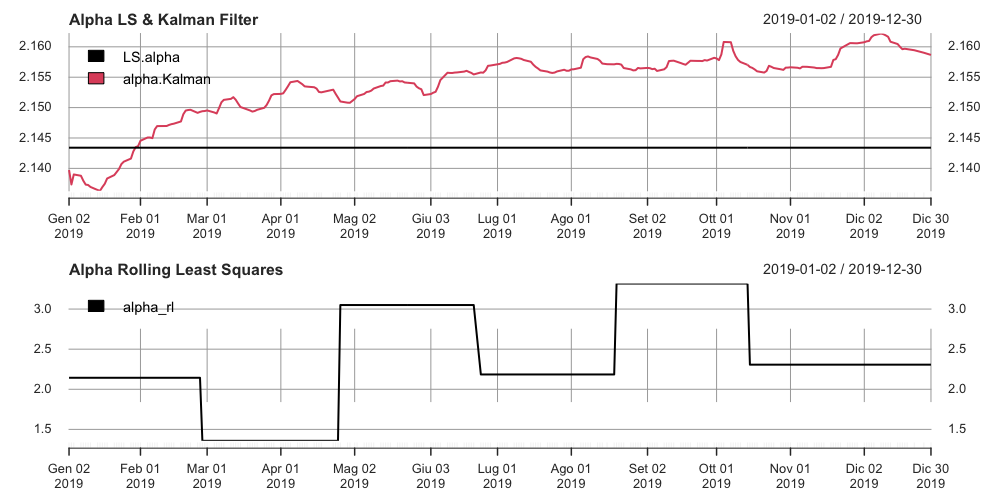
\includegraphics[scale=0.3]{alpha_dia_amp.png}
\end{figure}
\\
\begin{figure}[h]
	\caption{$\hat{\beta}$}
	\centering
	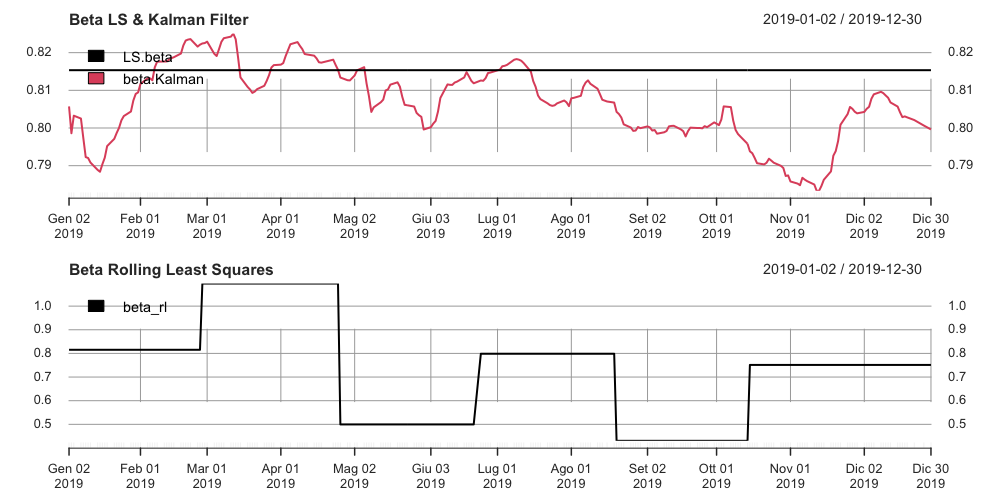
\includegraphics[scale=0.3]{beta_dia_amp.png}
\end{figure}
\\
Con i parametri ottenuti con i tre diversi approcci è stato calcolato poi lo spread come definito in (\ref{spread}).
Al fine di equiparare le 3 diverse metodologie, per la coppia \textbf{DIA.MI-AMP.MI} è stato scelto un valore soglia di 0.02.
\\
I \textbf{P\&L} delle tre diverse strategie sono visibili nella figura 4.
\\\\\\\\\\\\
Di seguito la valutazione delle tre performance:
% PERFORMANCE
\begin{center}
\captionof{table}{Performance evaluation}
\begin{tabular}{ p{3cm}p{2cm}p{1cm}p{1cm}p{2cm} }
	\hline
	Metodologia  & Sharpe Ratio & MDD & AR & RMSE\\
	\hline
	Kalman Filter & 1.85 & 0.02 & 0.16 & 0.013 \\
	Co-Integration & 3.45 & 0.05 & 0.42 & 0.037 \\
	Rolling Regression & 3.56 & 0.05 & 0.41 & 0.032 \\
	\hline
\end{tabular}
\end{center}
\
\\\\
\begin{figure}[h]
	\caption{$	z_t= log(stock_{1,t}) - \hat{\beta}log(stock_{2,t}) - \hat{\alpha}$}
	\centering
	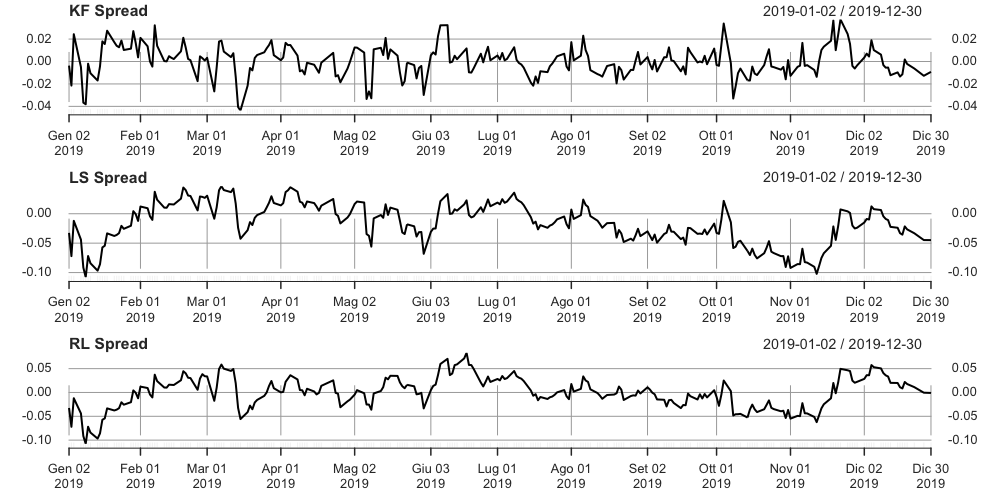
\includegraphics[scale=0.3]{spread_dia_amp.png}
\end{figure}

\begin{figure}[h]
	\caption{Portfolio P\&L}
	\centering
	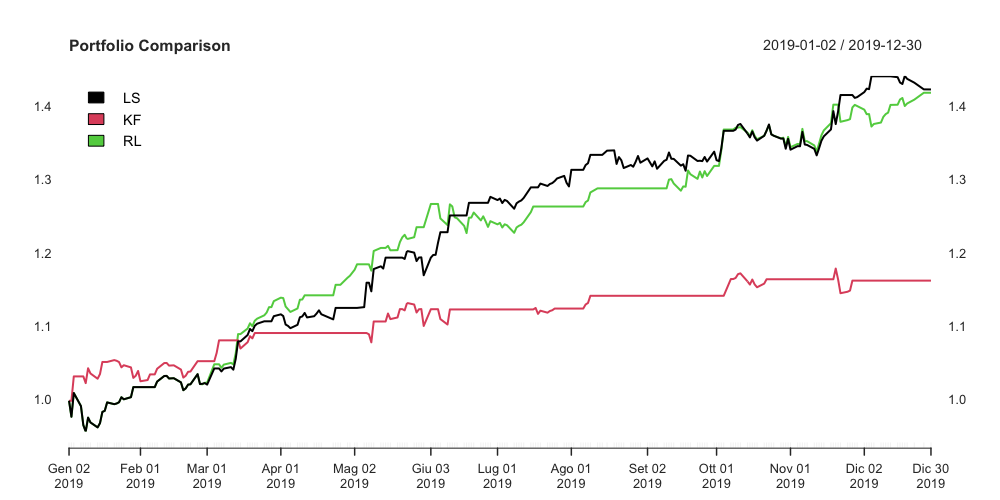
\includegraphics[scale=0.3]{comparison_dia_amp.png}
\end{figure}

\
\\\\\\\\\\\\
\begin{lstlisting}
#initial position
signal[1] <- 0
if (Z_score[1] <= threshold_long[1]) {
	signal[1] <- 1
} else if (Z_score[1] >= threshold_short[1])
signal[1] <- -1

# loop
for (t in 2:nrow(Z_score)) {
	if (signal[t-1] == 0) {  #if we were in no position
		if (Z_score[t] <= threshold_long[t]) {
			signal[t] <- 1
		} else if(Z_score[t] >= threshold_short[t]) {
			signal[t] <- -1
		} else signal[t] <- 0
	} else if (signal[t-1] == 1) {  #if we were in a long position
		if (Z_score[t] >= 0) signal[t] <- 0
		else signal[t] <- signal[t-1]
	} else {  #if we were in a short position
		if (Z_score[t] <= 0) signal[t] <- 0
		else signal[t] <- signal[t-1]
	}
}
\end{lstlisting}



\end{document}
